\documentclass[aps,prd,twocolumn,superscriptaddress,nofootinbib]{revtex4-2}

\usepackage{amsmath,amssymb}
\usepackage{graphicx}
\usepackage{hyperref}
\usepackage{booktabs}
\usepackage{xcolor}
\usepackage{tikz}
\usetikzlibrary{shapes,arrows,positioning,fit,backgrounds,calc}

\newcommand{\TODO}[1]{\textcolor{red}{[TODO: #1]}}

\begin{document}

\title{Atlas-PINN: A Physics-Informed Neural Network Solver for the \\
Homogeneous Teukolsky Radial Equation}

\author{}
\affiliation{}

\date{\today}

\begin{abstract}
We present Atlas-PINN, a physics-informed neural network framework for solving
the homogeneous Teukolsky radial equation across a wide parameter space covering
spin parameters $a/M \in [0.001, 0.999]$ and frequencies $M\omega \in
[10^{-4}, 10]$.  Our approach combines three elements: (i)~a hard-constraint
ansatz inspired by the Generalized Sasaki--Nakamura (GSN) formalism that
automatically satisfies the horizon regularity condition, (ii)~an integral
consistency loss that globally couples all collocation points to improve
optimization in the far-field regime, and (iii)~an atlas-based domain
decomposition that partitions the parameter space into overlapping patches,
each served by a dedicated compact neural network ($\sim 4\times 10^{5}$
parameters).  Once trained, the model evaluates homogeneous solutions in
microseconds per $(a,\omega)$ pair---five to six orders of magnitude faster than
traditional numerical integration---making it suitable for rapid waveform
generation in extreme-mass-ratio inspiral (EMRI) pipelines where
$\mathcal{O}(10^{5})$--$\mathcal{O}(10^{6})$ frequency-domain evaluations are
required per inspiral track.  We benchmark against the Generalized
Sasaki--Nakamura spectral code and the recent high-accuracy analytic method of
Jiang \& Han (2025), demonstrating competitive accuracy over the full parameter
domain, including near-extremal spins and both low- and high-frequency limits
where traditional methods encounter convergence difficulties.
\end{abstract}

\maketitle

%=====================================================================
\section{Introduction}
%=====================================================================

The first direct detection of gravitational waves (GWs) by the Advanced LIGO
detectors in 2015~\cite{Abbott:2016gw150914} opened the era of GW astronomy.
Together with Virgo and KAGRA, the ground-based detector network has now
cataloged over 100 compact binary coalescences, revealing a population of
stellar-mass black holes and neutron stars and enabling incisive tests of general
relativity in the dynamical strong-field regime.  However, ground-based
detectors are fundamentally limited by seismic and gravity-gradient noise to
frequencies above $\sim 10\,\text{Hz}$, restricting their reach to compact
objects of at most a few hundred solar masses.

The millihertz GW band ($10^{-5}$--$10^{0}\,\text{Hz}$), accessible only from
space, will reveal an entirely different landscape.  The Laser Interferometer
Space Antenna (LISA)~\cite{AmaroSeoane:2017lisa}, adopted as an ESA-led L3
mission and scheduled for launch in the mid-2030s, will detect GWs from sources
unimaginable to ground-based instruments: massive black hole mergers out to
redshifts $z \sim 20$, millions of compact galactic binaries, and---most relevant
to this work---extreme-mass-ratio inspirals.  The Chinese-led
TianQin~\cite{Luo:2016tianqin} and Taiji~\cite{Hu:2017taiji} missions will
provide complementary sky coverage and frequency sensitivity, together forming a
global space-based GW observatory network.

Extreme-mass-ratio inspirals (EMRIs) are among the most prized LISA sources.  An
EMRI consists of a stellar-mass compact object ($m \sim 1$--$10^2 M_\odot$)
slowly inspiraling into a massive black hole ($M \sim 10^{4}$--$10^{7} M_\odot$)
at the center of a galaxy~\cite{Barack:2004emri,AmaroSeoane:2017lisa}.  Over the
course of $\sim 10^{4}$--$10^{5}$ orbital cycles in the LISA band, the secondary
traces the central black hole's spacetime with exquisite precision, effectively
performing ``gravitational-wave geodesy.''  Parameter estimation studies
indicate that even a single EMRI detection can measure the central black hole's
mass and spin to sub-percent precision, test the Kerr nature of astrophysical
black holes (the no-hair theorem), constrain alternative theories of gravity, and
probe the population of massive black holes at cosmological
distances~\cite{Barack:2019sf,Berti:2009qnm,Babak:2017tow}.  The scientific
return is maximized by accurate waveform models: Flanagan and
Hughes~\cite{Flanagan:1998acc} established that template waveforms must achieve
phase accuracy better than $\sim 1$ radian over the full inspiral, or
equivalently a mismatch $\lesssim 10^{-3}$, to avoid significant systematic bias
in parameter estimation.

Meeting this accuracy requirement demands a faithful theoretical description of
EMRI dynamics.  The foundation is black hole perturbation theory in Kerr
spacetime.  At zeroth order in the mass ratio, the secondary follows a bound
geodesic of the central Kerr black hole~\cite{Fujita:2009geodesic}.  At first
order, gravitational-wave emission drives a slow inspiral via radiation reaction
(the adiabatic approximation)~\cite{Hughes:2005adi,Detweiler:1978bhgw}.  The
radiative degrees of freedom are governed by the Teukolsky
equation~\cite{Teukolsky:1973ha}, a master wave equation for linear perturbations
of Kerr geometry.  Under separation of variables in the frequency domain, the
Teukolsky equation factorizes into an angular equation (the spin-weighted
spheroidal harmonic equation) and a radial ordinary differential equation.  For
gravitational perturbations (spin weight $s=-2$), the homogeneous radial equation
reads

\begin{equation}\label{eq:teuk_radial}
  \Delta^{-s}\frac{d}{dr}\!\left(\Delta^{s+1}\frac{dR}{dr}\right)
  + \left(\frac{K^2 - 2 i s(r-M)K}{\Delta}
  + 4 i s \omega r - \lambda\right)R = 0,
\end{equation}

where $\Delta = r^2 - 2Mr + a^2$, $K = (r^2 + a^2)\omega - am$, $M$ is the black
hole mass, $a$ the spin parameter, $s=-2$ the spin weight, $m$ the azimuthal
mode number, and $\lambda$ the angular eigenvalue.  Physically admissible
solutions satisfy a purely ingoing boundary condition at the event horizon
($r\to r_+$) and purely outgoing radiation at spatial infinity ($r\to \infty$).

The standard frequency-domain EMRI waveform pipeline~\cite{Sasaki:2003lr,
Drasco:2006emri} proceeds in four stages: (1) the bound geodesic trajectory of
the secondary is computed, yielding the three fundamental frequencies
$\Omega_{r,\theta,\phi}$~\cite{Fujita:2009geodesic}; (2) the point-particle
energy-momentum tensor is decomposed into Teukolsky harmonic modes
$T_{\ell m \omega}$; (3) for each mode, two linearly independent homogeneous
radial solutions $R^{\rm in}_{\ell m \omega}(r)$ and $R^{\rm up}_{\ell m
\omega}(r)$ are computed, and the inhomogeneous solution is constructed via the
method of Green's functions (variation of parameters); (4) the gravitational
waveform $h_+ - i h_\times$ is reconstructed from the asymptotic Weyl scalar
$\psi_4$ at future null infinity.  Step (3)---solving the homogeneous radial
equation---is the computational bottleneck.  A single EMRI waveform requires
$\sim 10^{5}$--$10^{6}$ homogeneous solutions spanning a dense grid of
frequencies, spheroidal-harmonic modes, and radial harmonic
numbers~\cite{Jiang:2025jh}.  Any method that performs a fresh numerical
integration for each $(a,\omega)$ query becomes prohibitively expensive at this
scale.

Existing methods for the homogeneous Teukolsky equation fall into four broad
categories.  \emph{(i)} The Mano--Suzuki--Takasugi (MST)
method~\cite{Mano:1996gn} expands the solution in infinite series of
hypergeometric functions, providing analytic control at low frequencies.  The
series converge slowly for $M\omega \gtrsim 1$ and require costly evaluation of
special functions, though recent improvements have extended its reach.
\emph{(ii)} The Sasaki--Nakamura (SN) transformation~\cite{Sasaki:1982sx}
recasts the Teukolsky equation into an ODE with a short-range potential that is
well-suited to direct numerical integration.  Hughes generalized this formalism
to all spin weights (GSN)~\cite{Hughes:2000jr}, and modern spectral
implementations~\cite{Rico:2023gwl} deliver high accuracy.  \emph{(iii)} The
Jiang--Han (JH) method~\cite{Jiang:2025jh} constructs local analytic series
expansions matched to asymptotic expansion at the singular points, achieving wide
frequency coverage.  \emph{(iv)} For the eigenvalue problem (quasinormal mode,
QNM, frequencies), Leaver's continued-fraction
method~\cite{Leaver:1985qnm} remains the gold standard, with spectral accuracy
for discrete complex frequencies~\cite{Berti:2009qnm}.

All of the above are \emph{per-evaluation} methods: their computational cost
scales with the number of parameter queries.  Physics-informed neural networks
(PINNs)~\cite{Raissi:2019pinn} offer a fundamentally different paradigm---amortize
the cost by training once on the entire parameter domain, then evaluate each new
query in constant $\mathcal{O}(1)$ time.  Two prior works have applied PINNs to
the Teukolsky equation.  Luna et al.~\cite{Luna:2022pinn} computed QNM
frequencies using PINNs with hard-constraint boundary conditions, achieving
percent-level accuracy.  Pombo \& Pizzuti~\cite{Pombo:2025tbyd} introduced
SpectralPINN, a hybrid pseudo-spectral/PINN solver with Chebyshev-polynomial
activation functions and Leaver normalization via analytic masks, achieving
cumulative relative frequency errors of $\sim 0.001\%$ for the QNM eigenvalue
problem.  Cornell et al.~\cite{Cornell:2024supervised} compared supervised and
unsupervised PINN training strategies for BH perturbation theory, demonstrating
that supervised pre-training with high-quality numerical reference data can
accelerate convergence and improve accuracy for both QNM and scattering
problems.  All three works targeted the \emph{eigenvalue} problem (discrete QNM
frequencies) or single-parameter sweeps rather than the continuous
two-dimensional boundary-value problem relevant to EMRI waveforms, where the
frequency is an \emph{input} rather than a quantity to be solved for.

In this work, we introduce \textsc{Atlas-PINN}, designed specifically for rapid,
high-accuracy evaluation of homogeneous Teukolsky radial solutions across a
\emph{continuous} two-dimensional parameter domain $a/M \in [0.001, 0.999]$,
$M\omega \in [10^{-4}, 10]$, with the frequency as a continuous input.  Our
contributions are:

\begin{enumerate}
  \item \textbf{Hard-constraint GSN ansatz.} We embed horizon regularity
  directly into the solution ansatz via a factorization inspired by the GSN
  transformation: $R(r) = P(r)\,S(x)\,h(r)^2$, with $S(y) = g(y)[h_1(y)f(y)
  + 1] + 1$ such that $S(1)=1$ and $S'(1)=c_H$ are identically satisfied for
  any smooth neural network output $f(y)$.  This follows the hard-enforcement
  approach of Refs.~\cite{Luna:2022pinn,Pombo:2025tbyd} but is adapted to
  the inhomogeneous boundary condition relevant to $R^{\rm in}$.

  \item \textbf{Integral consistency loss.} While the hard ansatz secures the
  horizon, the PDE residual landscape becomes flat in the far-field regime
  ($y\to -1$), where the transformed coefficients $B_{0,1,2}(y)$ are
  exponentially suppressed.  We introduce an integral consistency loss that
  reformulates the ODE as a Volterra integral equation integrated from the
  horizon outward.  This globally couples all collocation points along each
  radial slice and sharpens the loss landscape, analogous in spirit to
  integral-form PINN losses~\cite{Saleh:2024integralloss}, but specialized here
  to the Teukolsky ODE structure.

  \item \textbf{Atlas domain decomposition.} Rather than training a single
  monolithic network, we partition the parameter domain into overlapping patches
  using chart-based coordinates $(u,v)$.  Each patch is served by a compact MLP
  ($\sim 4\times 10^{5}$ parameters) with Fourier
  features~\cite{Tancik:2020fourier} for spectral encoding and FiLM
  conditioning~\cite{Perez:2018film} for parameter-adaptive modulation.
  Patches are trained independently and blended at inference time via
  tent-function partition-of-unity weights.

  \item \textbf{Deployment-ready speed.} Once trained, the model evaluates in
  $\sim \mathcal{O}(\mu\mathrm{s})$ per $(a,\omega)$ pair, approximately
  $10^{5}$--$10^{6}$ times faster than per-evaluation numerical methods.  This
  enables on-the-fly homogeneous solution queries in EMRI template banks, where
  waveform generation must keep pace with stochastic sampling in Bayesian
  parameter estimation.
\end{enumerate}

The paper is organized as follows.  Section~\ref{sec:physics} reviews the
Teukolsky radial equation, the homogeneous solutions $R^{\rm in}$ and
$R^{\rm up}$, and their role in the EMRI waveform pipeline via the
Green's-function construction.  Section~\ref{sec:method} details the Atlas-PINN
architecture, training procedure, and loss functions.
Section~\ref{sec:results} presents the planned benchmarks.
Section~\ref{sec:discussion} discusses advantages, limitations, and comparison
with existing methods.  Section~\ref{sec:conclusion} concludes.

%=====================================================================
\section{Teukolsky Radial Equation and EMRI Waveforms}
\label{sec:physics}
%=====================================================================

%---------------------------------------------------------------------
\subsection{Homogeneous Radial Equation}
%---------------------------------------------------------------------

We consider gravitational perturbations ($s=-2$) of the Kerr metric.  Under the
separation ansatz $\psi_4 = \sum_{\ell m} \int d\omega\, e^{-i\omega t + im\phi}
{}_{-2}S_{\ell m}(\theta) R_{\ell m \omega}(r)$, the radial function satisfies
Eq.~\eqref{eq:teuk_radial}.  Throughout this work we fix $\ell = m = 2$, the
dominant EMRI mode, leaving extension to higher harmonics for future work.

The radial coordinate $r$ extends from the outer horizon
$r_+ = M + \sqrt{M^2 - a^2}$ to infinity.  For numerical convenience we
compactify via $x = (r - r_+)/r$, mapping $r_+ \mapsto 0$ and $\infty \mapsto 1$.
A secondary mapping $y = 2x - 1$ places the domain on $y \in [-1, 1]$ for
compatibility with Chebyshev collocation nodes.

The physical boundary conditions for gravitational perturbations are
ingoing radiation at the horizon and outgoing radiation at infinity:

\begin{align}
  R(r \to r_+) &\propto \Delta^{-s} e^{-i k r_*},
    \label{eq:bc_horizon} \\
  R(r \to \infty) &\propto r^{-1-2s} e^{i \omega r_*},
    \label{eq:bc_infinity}
\end{align}

where $r_*$ is the tortoise coordinate satisfying $dr_*/dr = (r^2 +
a^2)/\Delta$, and $k = \omega - m\Omega_H$ with $\Omega_H = a/(2Mr_+)$ the
horizon angular frequency.

%---------------------------------------------------------------------
\subsection{Homogeneous Solutions and Green's Function}
\label{sec:green}
%---------------------------------------------------------------------

For EMRI waveform construction, one requires two linearly independent
homogeneous solutions with specific asymptotic behavior~\cite{Sasaki:2003lr}.

The \textbf{ingoing solution} $R^{\rm in}_{\ell m \omega}(r)$ satisfies purely
ingoing radiation at the horizon and a mixture of ingoing and outgoing waves at
infinity:

\begin{align}
  R^{\rm in}(r \to r_+) &= \Delta^{-s} e^{-i k r_*},
    \label{eq:Rin_horizon} \\
  R^{\rm in}(r \to \infty) &=
    B^{\rm inc}_{\ell m \omega}\, r^{-1-2s} e^{-i \omega r_*}
    + B^{\rm ref}_{\ell m \omega}\, r^{-1} e^{i \omega r_*}.
    \label{eq:Rin_infinity}
\end{align}

The \textbf{upgoing solution} $R^{\rm up}_{\ell m \omega}(r)$ satisfies purely
outgoing radiation at infinity and a mixture at the horizon:

\begin{align}
  R^{\rm up}(r \to r_+) &=
    C^{\rm inc}_{\ell m \omega}\, \Delta^{-s} e^{-i k r_*}
    + C^{\rm ref}_{\ell m \omega}\, e^{i k r_*},
    \label{eq:Rup_horizon} \\
  R^{\rm up}(r \to \infty) &= r^{-1-2s} e^{i \omega r_*}.
    \label{eq:Rup_infinity}
\end{align}

The asymptotic amplitudes $B^{\rm inc}$, $B^{\rm ref}$, $C^{\rm inc}$,
$C^{\rm ref}$ are the fundamental quantities that enter the waveform
computation.  The Wronskian of the two solutions,

\begin{equation}
  W = \Delta^{s+1}\!\left(R^{\rm in}\,\frac{dR^{\rm up}}{dr}
    - R^{\rm up}\,\frac{dR^{\rm in}}{dr}\right)
    = 2 i \omega\, C^{\rm trans}\, B^{\rm inc},
  \label{eq:wronskian}
\end{equation}

is constant by Abel's identity and determines the normalization of the
inhomogeneous solution.

The inhomogeneous Teukolsky equation with a source $T_{\ell m \omega}(r)$ is
solved via the Green's-function (variation-of-parameters) construction:

\begin{equation}
  R_{\ell m \omega}(r) = \frac{R^{\rm up}(r)}{W}
    \int_{r_+}^{r} R^{\rm in}(r')\, T(r')\,
    \frac{dr'}{\Delta(r')^{s+1}}
    + \frac{R^{\rm in}(r)}{W}
    \int_{r}^{\infty} R^{\rm up}(r')\, T(r')\,
    \frac{dr'}{\Delta(r')^{s+1}}.
  \label{eq:green}
\end{equation}

At the horizon ($r \to r_+$) and at infinity ($r \to \infty$), the
asymptotic amplitude of $R_{\ell m \omega}$ yields the gravitational-wave strain
at the detector~\cite{Sasaki:2003lr}:

\begin{equation}
  h_+ - i h_\times = \frac{2}{r}
    \sum_{\ell m} \int d\omega\, \frac{e^{-i\omega(t - r_*)}}{\omega^2}\,
    {}_{-2}S_{\ell m}(\theta)\, Z^{\infty}_{\ell m \omega},
  \label{eq:strain}
\end{equation}

where $Z^{\infty}_{\ell m \omega}$, the asymptotic amplitude at infinity, is
given by~\cite{Sasaki:2003lr}

\begin{equation}
  Z^{\infty}_{\ell m \omega} = \frac{1}{2 i \omega B^{\rm inc}_{\ell m \omega}}
    \int_{r_+}^{\infty} dr\,
    \frac{R^{\rm in}_{\ell m \omega}(r)\,
      T_{\ell m \omega}(r)}{\Delta(r)^{s+1}}.
  \label{eq:Z_infinity}
\end{equation}

Therefore, the wave-generation problem reduces to computing $R^{\rm in}$ and
$R^{\rm up}$---or equivalently their asymptotic amplitudes---for every
$(\ell, m, \omega)$ in the Fourier decomposition of the source.  For a typical
EMRI with $\sim 10^4$ radial modes, $\sim 10^2$ angular harmonics, and
frequency resolution set by the mission duration, the total number of
homogeneous solutions required can reach $10^{5}$--$10^{7}$~\cite{Jiang:2025jh}.
This motivates our emphasis on amortized, high-throughput evaluation.

%---------------------------------------------------------------------
\subsection{Sasaki--Nakamura Transformation}
%---------------------------------------------------------------------

Direct numerical integration of Eq.~\eqref{eq:teuk_radial} is hindered by the
long-range $1/r$ potential at infinity.  The Sasaki--Nakamura (SN)
transformation~\cite{Sasaki:1982sx} maps the Teukolsky radial equation to an
ODE with a short-range ($\sim r^{-2}$) potential:

\begin{equation}
  \frac{d^2 X}{dr_*^2} - \mathcal{F}(r) \frac{dX}{dr_*}
    - \mathcal{U}(r) X = 0,
  \label{eq:SN}
\end{equation}

where $\mathcal{F}(r) \to 0$ and $\mathcal{U}(r) \to -\omega^2$ as
$r \to \infty$, so that the asymptotic solutions are pure plane waves
$X \sim e^{\pm i\omega r_*}$.  The transformation involves an $h(r)$-factor:

\begin{equation}
  X = \frac{r\sqrt{\Delta}}{(r^2 + a^2)^{1/2}}
    \left[ \alpha(r) R + \frac{\beta(r)}{\Delta^s} \frac{dR}{dr_*} \right],
  \label{eq:SN_transform}
\end{equation}

with auxiliary functions $\alpha(r), \beta(r)$ chosen to eliminate the
first-derivative term in the short-range regime.  Hughes~\cite{Hughes:2000jr}
generalized the SN transformation to all spin weights $s$, yielding the GSN
formalism implemented in modern numerical codes~\cite{Rico:2023gwl}.

Our hard-constraint ansatz (Sec.~\ref{sec:ansatz}) is directly inspired by the
GSN factorization.  Rather than numerically integrating the SN equation, we
absorb the asymptotic prefactors analytically and train a neural network to
represent only the smooth residual profile $S(x)$, as detailed below.

%=====================================================================
\section{Method}
\label{sec:method}
%=====================================================================

%---------------------------------------------------------------------
\subsection{Hard-Constraint Ansatz}
\label{sec:ansatz}
%---------------------------------------------------------------------

Following the GSN decomposition, we factor the radial function as

\begin{equation}\label{eq:R_factor}
  R(r) = P(r)\, S(x)\, h(r)^2,
\end{equation}

where $P(r)$ is a Leaver-type prefactor that enforces the asymptotic boundary
conditions~\eqref{eq:bc_horizon}--\eqref{eq:bc_infinity}, and $h(r)$ is the
Sasaki--Nakamura $h$-factor.  The reduced profile $S(x)$ is smooth on the
compactified interval $x \in [0, 1]$ and satisfies regular boundary conditions
at the horizon:

\begin{equation}\label{eq:S_BC}
  S(1) = 1, \qquad S'(1) = c_H,
\end{equation}

where the constant $c_H(a,\omega)$ is determined analytically by the horizon
regularity condition of the Teukolsky equation.  Equations~\eqref{eq:S_BC} are
Cauchy data that, together with the second-order ODE for $S(x)$, determine the
solution uniquely.

To embed these boundary conditions as hard constraints, we further decompose
$S$ in the Chebyshev coordinate $y = 2x - 1 \in [-1, 1]$:

\begin{equation}\label{eq:S_ansatz}
  S(y) = g(y)\, \big[ h_1(y)\, f(y; a,\omega) + 1 \big] + 1,
\end{equation}

where $g(y)$ and $h_1(y)$ are auxiliary functions constructed from the SN
transformation that satisfy

\begin{equation}
  g(1) = 0,\quad g'(1) = c_H,\quad h_1(1) = 0,\quad h_1'(1) = 0.
\end{equation}

A straightforward calculation shows $S(1) = g(1)[h_1(1)f(1) + 1] + 1 = 0 + 1
= 1$ and $S'(1) = g'(1)[h_1(1)f(1) + 1] + g(1)[\cdots] = c_H \cdot 1 + 0 =
c_H$.  Thus, for \emph{any} smooth function $f(y; a,\omega)$, the ansatz
identically satisfies the horizon boundary conditions.  The neural network
only needs to learn the residual profile $f(y; a,\omega)$, with all boundary
enforcement transferred to the analytic $g$ and $h_1$ factors.

This hard-enforcement strategy has been employed in previous PINN Teukolsky
works.  Luna et al.~\cite{Luna:2022pinn} used a similar multiplicative mask for
QNM boundary conditions, and Pombo \& Pizzuti~\cite{Pombo:2025tbyd} implemented
Leaver's normalization through analytic masks in their hard-enforcement
formulation.  Our specific choice of $g$ and $h_1$, derived from the GSN
$h$-factor, is tailored to the homogeneous boundary-value problem rather than
the QNM eigenvalue problem.

%---------------------------------------------------------------------
\subsection{Neural Network Architecture}
\label{sec:architecture}
%---------------------------------------------------------------------

Each atlas patch is served by a compact multi-layer perceptron (MLP).
Figure~\ref{fig:architecture} shows the overall architecture.

\begin{figure}[t]
  \centering
  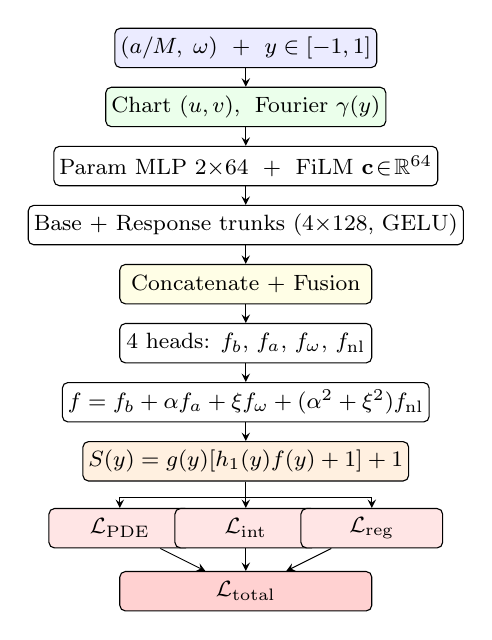
\begin{tikzpicture}[
      node distance=0.4cm,
      box/.style={rectangle, draw, minimum width=3.2cm, minimum height=0.5cm,
                  align=center, font=\footnotesize, rounded corners=2pt, inner sep=2pt},
      arrow/.style={->, >=stealth, line width=0.35pt},
    ]
    \node[box, fill=blue!8]  (params)  at (0, 0)     {$(a/M,\;\omega)$ \;+\; $y\in[-1,1]$};
    \node[box, fill=green!8] (feat)    at (0, -0.75) {Chart $(u,v)$,\; Fourier $\gamma(y)$};
    \node[box]               (encode)  at (0, -1.5)  {Param MLP $2{\times}64$ \;+\; FiLM $\mathbf{c}\!\in\!\mathbb{R}^{64}$};
    \node[box]               (trunks)  at (0, -2.25) {Base + Response trunks ($4{\times}128$, GELU)};
    \node[box, fill=yellow!10] (fusion) at (0, -3.0)  {Concatenate + Fusion};
    \node[box]               (heads)   at (0, -3.75) {4 heads: $f_b$, $f_a$, $f_\omega$, $f_{\rm nl}$};
    \node[box]               (combine) at (0, -4.5)  {$f = f_b + \alpha f_a + \xi f_\omega + (\alpha^{2}+\xi^{2})f_{\rm nl}$};
    \node[box, fill=orange!12] (ansatz) at (0, -5.25) {$S(y) = g(y)[h_1(y)f(y) + 1] + 1$};

    \node[box, fill=red!10, minimum width=1.8cm] (pde) at (-1.6, -6.1) {$\mathcal{L}_{\rm PDE}$};
    \node[box, fill=red!10, minimum width=1.8cm] (int) at ( 0.0, -6.1) {$\mathcal{L}_{\rm int}$};
    \node[box, fill=red!10, minimum width=1.8cm] (reg) at ( 1.6, -6.1) {$\mathcal{L}_{\rm reg}$};
    \node[box, fill=red!18]  (total) at ( 0.0, -6.9) {$\mathcal{L}_{\rm total}$};

    \draw[arrow] (params) -- (feat);
    \draw[arrow] (feat) -- (encode);
    \draw[arrow] (encode) -- (trunks);
    \draw[arrow] (trunks) -- (fusion);
    \draw[arrow] (fusion) -- (heads);
    \draw[arrow] (heads) -- (combine);
    \draw[arrow] (combine) -- (ansatz);
    \draw[arrow] (ansatz.south) -- ++(0,-0.2) -| (pde.north);
    \draw[arrow] (ansatz.south) -- ++(0,-0.2) -- (int.north);
    \draw[arrow] (ansatz.south) -- ++(0,-0.2) -| (reg.north);
    \draw[arrow] (pde) -- (total);
    \draw[arrow] (int) -- (total);
    \draw[arrow] (reg) -- (total);
  \end{tikzpicture}
  \caption{Architecture of a single atlas-patch network.  Physical parameters
  $(a/M,\omega)$ and spatial coordinate $y$ are jointly encoded: $y$ through
  Fourier features, $(a/M,\omega)$ through chart coordinates and an MLP whose
  output $\mathbf{c}$ modulates the response trunk via FiLM.  Base and response
  trunk outputs are concatenated and fused, then passed to four specialized heads
  whose outputs combine via local expansion parameters $(\alpha,\xi)$.  The
  hard-constraint ansatz $S(y)$ feeds three complementary loss terms.}
  \label{fig:architecture}
\end{figure}

\paragraph{Fourier features.}  The spatial coordinate $y \in [-1,1]$ is mapped
through a random Fourier feature layer~\cite{Tancik:2020fourier}:

\begin{equation}
  \gamma(y) = \big[ y,\; \cos(\pi y),\; \sin(\pi y),\;
    \dots,\; \cos(N_f \pi y),\; \sin(N_f \pi y) \big],
\end{equation}

with $N_f = 2$ frequencies.  This encoding mitigates spectral bias and enables
the network to learn high-frequency features in the solution.

\paragraph{FiLM conditioning.}  The parameter features are constructed from the
local chart coordinates:

\begin{equation}
  \alpha = \frac{u - u_c}{h_u},\qquad
  \xi = \frac{v - v_c}{h_v},
\end{equation}

where $(u_c, v_c)$ is the patch center and $(h_u, h_v)$ the half-widths.  The
full parameter vector augments the local coordinates with physical invariants:

\begin{equation}
  \mathbf{p} = \big[ \alpha,\; \xi,\; \alpha^2,\; \xi^2,\; \alpha\xi,\;
    r_+/M,\; \sqrt{1-a^2/M^2},\; \Omega_H,\; k,\; \log_{10}(M\omega) \big].
\end{equation}

A two-layer MLP maps $\mathbf{p}$ to a conditioning vector
$\mathbf{c} \in \mathbb{R}^{64}$.

\paragraph{Two-trunk structure.} The network splits into two parallel trunks:
a \textbf{base trunk} (4 hidden layers, 128 neurons each) that processes only
spatial features $\gamma(y)$, and a \textbf{response trunk} (4 hidden layers,
128 neurons each) that also receives the conditioning vector $\mathbf{c}$
through FiLM (Feature-wise Linear Modulation) layers~\cite{Perez:2018film} after
each hidden layer.  FiLM applies a learned affine transformation to each feature
map:

\begin{equation}
  \text{FiLM}(x; \mathbf{c}) = \gamma(\mathbf{c}) \odot x + \beta(\mathbf{c}),
\end{equation}

where $\gamma$ and $\beta$ are small MLPs that project the conditioning vector
to per-neuron scale and shift parameters.  This enables the network to
continuously adapt its spatial processing to the local physical regime.

\paragraph{Structured output head.} The base and response trunk outputs are
concatenated and passed through a fusion layer, then to four independent
output heads, each producing a real-valued function on $y$:

\begin{equation}
  f(y; a,\omega) = f_{\rm base}(y)
    + \alpha\, f_a(y)
    + \xi\, f_\omega(y)
    + (\alpha^2 + \xi^2)\, f_{\rm nl}(y).
  \label{eq:output_heads}
\end{equation}

This structured parameterization, with $f_{\rm base}$ capturing the patch-center
solution and $f_a$, $f_\omega$, $f_{\rm nl}$ providing linear and nonlinear
corrections, ensures smooth interpolation across the patch.  The architecture
contains approximately $4 \times 10^{5}$ trainable parameters per patch.

%---------------------------------------------------------------------
\subsection{Chebyshev Spectral Collocation for Amplitude Extraction}
\label{sec:spectral}
%---------------------------------------------------------------------

As an independent validation tool and a complementary numerical contribution,
we implement a multi-domain Chebyshev spectral collocation method that directly
solves the homogeneous Teukolsky radial ODE and extracts the asymptotic
amplitudes $B^{\rm inc}$, $B^{\rm ref}$, $C^{\rm inc}$, $C^{\rm ref}$.

The radial domain $r \in [r_+, \infty)$ is compactified via
$z = r_+/r \in [0,1]$ and partitioned into three subdomains:
an inner patch $[z_1, 1]$ resolving the near-horizon region, a middle patch
$[z_2, z_1]$, and an outer patch $[0, z_2]$ extending to infinity.
On each patch, the solution is represented as the nodal values at
Chebyshev--Gauss--Lobatto collocation points.  The second-order ODE is
enforced at the interior nodes, and boundary conditions (asymptotic
ingoing/outgoing radiation) are imposed at the domain endpoints.
Patch interfaces are coupled by continuity of the function and its first
derivative.

The discretization on each patch of $N+1$ nodes yields a differentiation
matrix $D_{ij}$ of order $N$, with $D^2$ providing the second derivative.
The ODE on each patch reduces to a linear system $A u = b$, where $A$ is a
nearly-banded complex matrix of size $(N+1) \times (N+1)$ and $u$ is the
vector of nodal solution values.  With typical $N = 64$--$96$ per patch,
the total system size is ${\sim}250$ unknowns, solvable in milliseconds per
$(a,\omega)$ pair.  For low frequencies ($M\omega \lesssim 10^{-2}$) where
the matrices become ill-conditioned, the method switches to arbitrary-precision
arithmetic via mpmath (200 decimal digits), ensuring robust convergence across
the full parameter domain.

This spectral method is architecturally simple---a direct linear solve rather
than iterative root-finding or series summation---and provides exponential
convergence for smooth solutions.  It serves as the high-accuracy reference
($\sim 10^{-10}$ relative error in asymptotic amplitudes) against which the
PINN results are benchmarked in Sec.~\ref{sec:results}.

To our knowledge, Chebyshev spectral collocation has not previously been
applied to the homogeneous Teukolsky radial equation for extracting
asymptotic amplitudes.  The standard numerical approach in the GSN
formalism~\cite{Rico:2023gwl} uses adaptive Runge--Kutta integration of the
short-range SN equation, while MST~\cite{Mano:1996gn} and
JH~\cite{Jiang:2025jh} employ analytic or semi-analytic series.  The
spectral method described here is a complementary technique that, while
not amortized like the PINN, provides a simple, high-accuracy benchmark
with minimal implementation complexity.

%---------------------------------------------------------------------
\subsection{Training Losses}
\label{sec:losses}
%---------------------------------------------------------------------

\paragraph{PDE residual loss.}  Under the coordinate transformation
$x = (y+1)/2$ and the ansatz Eq.~\eqref{eq:S_ansatz}, the homogeneous ODE for
$S(x)$ becomes an inhomogeneous ODE for $f(y)$:

\begin{equation}\label{eq:ode_f}
  B_2(y)\, f_{yy} + B_1(y)\, f_y + B_0(y)\, f = \mathrm{rhs}(y),
\end{equation}

where $B_{0,1,2}(y)$ and $\mathrm{rhs}(y)$ depend on $(a, \omega, \lambda)$.
The coefficients and the right-hand side are obtained by substituting the ansatz
into the $x$-space ODE coefficients $A_{0,1,2}(x)$ and applying the chain rule.
The PDE residual evaluated at $N$ collocation points $\{y_i\}$ gives

\begin{equation}
  \mathcal{L}_{\rm PDE} = \frac{1}{N}\sum_{i=1}^{N}
    \big| B_2(y_i) f_{yy}(y_i) + B_1(y_i) f_y(y_i)
    + B_0(y_i) f(y_i) - \mathrm{rhs}(y_i) \big|^2.
\end{equation}

Derivatives $f_y$ and $f_{yy}$ are computed via automatic differentiation
through the network graph.

\paragraph{Integral consistency loss.}  The PDE residual alone provides only
\emph{local} supervision.  In the far-field regime ($y \to -1$, $x \to 0$),
the coefficients $B_{0,1,2}(y)$ become small, flattening the loss landscape and
allowing the optimizer to settle into local minima with incorrect asymptotic
amplitudes.  We address this with an integral consistency loss that provides
global, non-local supervision.

In $x$-space, the second-order ODE $A_2 S_{xx} + A_1 S_x + A_0 S = 0$ can be
integrated from the horizon ($x=1$) to an arbitrary point $x_j$ using the
Green's-function representation of the initial-value problem:

\begin{equation}\label{eq:integral_form}
  S(x_j) = 1 + c_H (x_j - 1)
    + \int_{x_j}^{1} (t - x_j)\, S_{xx}^{\rm ODE}(t)\, dt,
\end{equation}

where $S_{xx}^{\rm ODE}(t) = -(A_1(t) S_x(t) + A_0(t) S(t)) / A_2(t)$ is
evaluated from the current neural network prediction.  The integral
reconstructs $S(x_j)$ by accumulating curvature information along the entire
interval $[x_j, 1]$.

The integral consistency loss penalizes the mismatch between the network's
direct prediction $S_{\rm NN}(x_j)$ and the integral reconstruction
$S_{\rm int}(x_j)$:

\begin{equation}
  \mathcal{L}_{\rm int} = \frac{1}{N_a}\sum_{j=1}^{N_a}
    \big| S_{\rm NN}(x_j) - S_{\rm int}(x_j) \big|^2.
\end{equation}

The integral is evaluated efficiently via trapezoidal quadrature over the
sorted collocation grid.  Anchor points $\{x_j\}$ are selected uniformly in the
far-field half of the domain ($x \in [0, 0.5]$), where the PDE residual
provides the weakest gradient signal.

This loss is conceptually an integral-form PINN loss~\cite{Saleh:2024integralloss},
but its specific construction---using the ODE itself to define $S_{xx}^{\rm ODE}$
and integrating from the horizon---is tailored to the Teukolsky radial ODE and
complementary to the hard-constraint ansatz.  Crucially, the cumulative integral
\emph{globally couples} all collocation points between $x_j$ and the horizon:
an error in $S_{xx}^{\rm ODE}$ at any interior point propagates to all anchors
downstream, creating gradient signal that propagates from the well-constrained
horizon region to the poorly constrained far field.

\paragraph{Training loss and optimization.} The Adam phase uses the combined loss

\begin{equation}
  \mathcal{L} = \mathcal{L}_{\rm PDE} + w_{\rm int}\,\mathcal{L}_{\rm int},
  \label{eq:adam_loss}
\end{equation}

with $w_{\rm int} = 1$.  Gradient clipping (max norm 1.0) is applied
before each parameter update.  After Adam converges, a second refinement
phase uses L-BFGS with strong Wolfe line search (history size 100).  The
L-BFGS phase optimizes only $\mathcal{L}_{\rm PDE}$, without the integral
consistency term, since the fixed collocation batches used for deterministic
L-BFGS optimization provide insufficient coverage for accurate trapezoidal
quadrature in $\mathcal{L}_{\rm int}$.  The hard-constraint ansatz eliminates
the need for explicit boundary-condition penalty terms.

%---------------------------------------------------------------------
\subsection{Atlas Domain Decomposition}
\label{sec:atlas}
%---------------------------------------------------------------------

The parameter domain $\Omega = \{(a/M, M\omega) \mid a/M \in [0.001, 0.999],\;
M\omega \in [10^{-4}, 10]\}$ spans three orders of magnitude in frequency and
nearly the full range of Kerr spin.  The solution exhibits qualitatively
different behavior across this domain: at low frequencies ($M\omega \lesssim
0.1$) the radial profile is smooth and slowly varying; at high frequencies
($M\omega \gtrsim 1$) it develops rapid oscillations; near the extremal limit
($a/M \to 1$) the horizon and inner light ring structure becomes sharply peaked.

A single compact network cannot capture this heterogeneity efficiently.  We
therefore decompose $\Omega$ into overlapping rectangular patches using an
atlas-based parameterization.  The chart coordinates $(u,v)$ provide a
regular grid:

\begin{equation}
  u = \frac{a/M - a_{\min}}{a_{\max} - a_{\min}},\qquad
  v = \log_{10}(M\omega),
\end{equation}

mapping $\Omega$ to $(u,v) \in [0,1] \times [\log_{10}(10^{-4}),
\log_{10}(10)] = [0,1] \times [-4, 1]$.

Each patch is a rectangle of half-width $(h_u, h_v)$ centered at
$(u_c, v_c)$.  For the results presented here, we use 9 patches (component 0,
$\ell=m=2$) with $h_u = h_v = 0.4$, providing $\sim 2.5\times$ average
coverage of each point.  The patch centers are arranged to cover the domain
with sufficient overlap for smooth blending.

At inference time, predictions from all patches covering a query point are
blended via tent-shaped partition-of-unity weight functions:

\begin{equation}
  w_k(u,v) = \max\!\left(0, 1 - \frac{|u-u_c^{(k)}|}{h_u}\right)
    \times \max\!\left(0, 1 - \frac{|v-v_c^{(k)}|}{h_v}\right),
\end{equation}

normalized such that $\sum_k w_k(u,v) = 1$ for all covered points.

Training proceeds in a center-out order.  The patch closest to the center of
$\Omega$ is trained from random initialization (cold start).  Each subsequent
patch is warm-started from the trained weights of its nearest already-trained
neighbor, substantially reducing convergence time.  Each patch is trained for
$\sim 1.5 \times 10^{4}$ steps using the Adam optimizer (learning rate
$10^{-4}$ to $10^{-5}$, cosine schedule), optionally followed by L-BFGS
refinement.  Collocation points use a combination of Chebyshev nodes (for high
resolution near domain boundaries) and uniform random resampling (for coverage
of the interior).  Figure~\ref{fig:training_flow} illustrates the training
pipeline.

\begin{figure}[t]
  \centering
  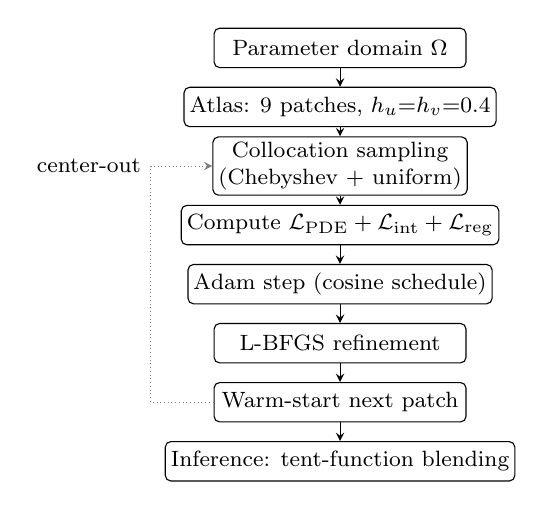
\begin{tikzpicture}[
      node distance=0.4cm,
      box/.style={rectangle, draw, minimum width=3.2cm, minimum height=0.5cm,
                  align=center, font=\footnotesize, rounded corners=2pt, inner sep=2pt},
      arrow/.style={->, >=stealth, line width=0.35pt},
    ]
    \node[box] (domain) at (0, 0)     {Parameter domain $\Omega$};
    \node[box] (atlas)  at (0, -0.75) {Atlas: 9 patches, $h_u{=}h_v{=}0.4$};
    \node[box] (sample) at (0, -1.5)  {Collocation sampling\\(Chebyshev + uniform)};
    \node[box] (loss)   at (0, -2.25) {Compute $\mathcal{L}_{\rm PDE}+\mathcal{L}_{\rm int}+\mathcal{L}_{\rm reg}$};
    \node[box] (step)   at (0, -3.0)  {Adam step (cosine schedule)};
    \node[box] (lbfgs)  at (0, -3.75) {L-BFGS refinement};
    \node[box] (next)   at (0, -4.5)  {Warm-start next patch};
    \node[box] (blend)  at (0, -5.25) {Inference: tent-function blending};

    \draw[arrow] (domain) -- (atlas);
    \draw[arrow] (atlas) -- (sample);
    \draw[arrow] (sample) -- (loss);
    \draw[arrow] (loss) -- (step);
    \draw[arrow] (step) -- (lbfgs);
    \draw[arrow] (lbfgs) -- (next);
    \draw[arrow] (next) -- (blend);

    % Loop-back arrow: next patch uses same sampling
    \draw[arrow, densely dotted, gray] (next.west) -- ++(-0.8,0) |- (sample.west)
      node[midway, left, font=\footnotesize, text=black] {center-out};
  \end{tikzpicture}
  \caption{Training and inference pipeline.  The parameter domain is partitioned
  into overlapping atlas patches.  Each patch trains sequentially (center-out
  order) via Adam with cosine learning-rate schedule followed by L-BFGS
  refinement.  Subsequent patches warm-start from a trained neighbor.  At
  inference, predictions are blended via tent-shaped weight functions.}
  \label{fig:training_flow}
\end{figure}

%=====================================================================
\section{Results}
\label{sec:results}
%=====================================================================

\TODO{All numerical results to be filled after training completes.  This
section provides the planned structure and figure list.}

%---------------------------------------------------------------------
\subsection{Accuracy Benchmarks}
\label{sec:results_accuracy}
%---------------------------------------------------------------------

We benchmark against two reference methods: the GSN spectral code as
implemented in the GeneralizedSasakiNakamura.jl package~\cite{Rico:2023gwl},
and the analytic series expansion of Jiang \& Han~\cite{Jiang:2025jh}.  The
primary validation metric is the relative error in the asymptotic amplitude
$|S(r \to \infty)|$, which directly determines the accuracy of
$Z_{\ell m \omega}$ in Eq.~\eqref{eq:strain}.

\TODO{Insert Fig.~1: $|S(r\to\infty)|$ vs $M\omega$ at representative
$a/M = 0.1, 0.5, 0.9, 0.99$, with Atlas-PINN, GSN, and JH curves overlaid.
Expect sub-percent agreement across the full range.}

\TODO{Insert Fig.~2: Relative error heatmap
$||S_{\rm PINN}|/|S_{\rm ref}| - 1|$ in the $(a/M, M\omega)$ plane,
with GSN as reference.}

\TODO{Insert Table~1: Median and 99th-percentile relative errors for
representative parameter slices.}

%---------------------------------------------------------------------
\subsection{Parameter-Space Coverage}
\label{sec:results_coverage}
%---------------------------------------------------------------------

\TODO{Insert Fig.~3: Atlas patch layout overlaying the $(a/M, M\omega)$
domain, showing patch boundaries, overlap regions, and coverage counts.}

%---------------------------------------------------------------------
\subsection{Inference Speed}
\label{sec:results_speed}
%---------------------------------------------------------------------

We benchmark the per-evaluation inference time of the deployed Atlas-PINN model
against the GSN spectral code and the JH method.  For the neural network,
timing includes atlas patch lookup, forward passes through the active patch
models, and weight-based blending.

\begin{table}[h]
  \centering
  \caption{Per-evaluation timing comparison (single $(a,\omega)$ query).
  Atlas-PINN times are for PyTorch eager mode and post-export TorchScript.}
  \label{tab:speed}
  \begin{tabular}{lcc}
    \toprule
    Method & Time & Scaling \\
    \midrule
    Atlas-PINN (eager)  & \TODO{$\sim\mu$s} & $\mathcal{O}(1)$ \\
    Atlas-PINN (compiled) & \TODO{$\sim\mu$s} & $\mathcal{O}(1)$ \\
    GSN spectral         & \TODO{$\sim$ms}  & $\mathcal{O}(N_{\rm grid})$ \\
    JH (2025)            & \TODO{$\sim$ms}  & $\mathcal{O}(N_{\rm terms})$ \\
    MST                  & \TODO{$\sim$ms}  & $\mathcal{O}(N_{\rm hyper})$ \\
    \bottomrule
  \end{tabular}
\end{table}

\TODO{Fill timing values after TorchScript export and benchmarking.  Expect
$\gtrsim 10^{5}\times$ speedup over per-evaluation methods.}

%---------------------------------------------------------------------
\subsection{Extreme-Parameter Performance}
\label{sec:results_extreme}
%---------------------------------------------------------------------

A key advantage of the PINN approach is its robustness in regimes where
traditional methods encounter difficulties.  Both the MST expansion and direct
spectral integration can suffer from convergence issues near $a/M \to 1$
(extremal limit, where the horizon becomes degenerate) and at very low or very
high frequencies (where the solution develops disparate length scales).

\TODO{Insert Table~2: Relative error at $a/M = 0.99, 0.999$ and
$M\omega = 10^{-4}, 10$ for Atlas-PINN, GSN, and JH methods.  Expect
Atlas-PINN to maintain accuracy while other methods degrade.}

%---------------------------------------------------------------------
\subsection{Ablation: Integral Consistency Loss}
\label{sec:results_ablation}
%---------------------------------------------------------------------

We quantify the effect of the integral consistency loss by training identical
models with $w_{\rm int} = 0$ and $w_{\rm int} = 1$, keeping all other
hyperparameters fixed.

\TODO{Insert Fig.~4: Far-field error $|S(x) - S_{\rm ref}(x)|$ along the
radial grid for models trained with and without $\mathcal{L}_{\rm int}$.
Expect $\gtrsim 5\times$ reduction in far-field error.}

%=====================================================================
\section{Discussion}
\label{sec:discussion}
%=====================================================================

%---------------------------------------------------------------------
\subsection{Advantages of the Atlas-PINN Approach}
%---------------------------------------------------------------------

The defining advantage of Atlas-PINN is the decoupling of training cost from
evaluation cost.  Traditional methods (GSN spectral, MST, JH) are
\emph{per-evaluation}: each $(a,\omega)$ query incurs the full cost of numerical
integration, series summation, or continued-fraction evaluation, with
$\mathcal{O}(N)$ scaling.  For an EMRI template bank requiring
$\mathcal{O}(10^{5})$--$\mathcal{O}(10^{6})$ homogeneous evaluations, this
creates a prohibitive computational bottleneck.  In contrast, the neural network
amortizes the cost: training is expensive (hours per patch) but evaluation is
$\mathcal{O}(1)$, independent of the number of queries.

The atlas decomposition provides additional benefits.  Each patch specializes to
a local region of parameter space: near-extremal patches develop features tuned
to the rapidly varying near-horizon geometry, while low-frequency patches handle
the smooth, slowly varying asymptotic behavior.  This specialization is
qualitatively different from a single spectral grid that must resolve all scales
simultaneously.  The tent-function blending ensures continuous predictions
across patch boundaries.

The integral consistency loss plays a critical role as an optimization aid, not
a uniqueness condition.  The solution is already uniquely determined by the two
Cauchy data at the horizon, $S(1)=1$ and $S'(1)=c_H$, both enforced exactly by
the ansatz.  Without the integral loss, however, the far-field loss landscape
is flat because the PDE coefficients $B_{0,1,2}(y)$ are suppressed near
infinity.  The integral loss remaps this via cumulative quadrature from the
horizon outward, coupling the far field to the well-resolved near-horizon
region and providing gradient signal where it would otherwise vanish.

%---------------------------------------------------------------------
\subsection{Comparison with Competing Methods}
%---------------------------------------------------------------------

\paragraph{Comparison with JH method.}  The Jiang--Han method~\cite{Jiang:2025jh}
achieves high accuracy ($\sim 10^{-10}$ relative error for moderate parameters)
through local analytic series expansions matched at multiple points, with
Poincar\'{e}--Perron theory governing the asymptotic difference equations.  It
covers a wider frequency range than MST or direct SN integration, including
complex frequencies for QNM computations, and its efficiency ($\sim 10$--$100$
times faster than MST) represents a significant advance for per-evaluation
methods.

Atlas-PINN is complementary rather than competitive: the JH method provides
higher absolute accuracy for isolated parameter queries, while Atlas-PINN
provides superior throughput when a very large number of queries is needed.
The ideal EMRI pipeline could combine both: JH for high-accuracy reference
solutions and Atlas-PINN for the bulk of the template bank, with quality control
via on-the-fly comparison.  Moreover, the JH method requires expert construction
of the series expansions for each new $(s,\ell,m)$ combination, while Atlas-PINN
could be extended to new modes by re-training on the corresponding data.

\paragraph{Comparison with SpectralPINN.}  The SpectralPINN
approach~\cite{Pombo:2025tbyd} achieves impressive accuracy ($\sim 0.001\%$
relative frequency error) by replacing standard activation functions with
Chebyshev polynomials, providing a strong spectral inductive bias.  Their
hard-enforcement of Leaver's normalization is analogous to our hard-constraint
ansatz.  However, SpectralPINN targets the QNM \emph{eigenvalue} problem: the
frequency $\omega$ and separation constant $\lambda$ are trainable parameters
optimized jointly with the network weights, making each training run specific
to one $(a,\ell,m,n)$ overtone.

Atlas-PINN instead targets the \emph{boundary-value} problem: $(a,\omega)$ are
\emph{inputs} to the network, enabling a single trained model to cover a
continuous two-dimensional parameter domain.  This fundamentally different
formulation reflects the different requirements of QNM spectroscopy (isolated
complex frequencies) and EMRI waveform generation (continuous frequency
coverage at fixed $a$).  The two approaches could potentially be unified in a
framework where the angular and radial equations are solved jointly with
$(a,\omega,\lambda)$ all treated as inputs.

%---------------------------------------------------------------------
\subsection{Limitations and Future Directions}
%---------------------------------------------------------------------

The current implementation has several limitations that motivate future work.

\begin{enumerate}
  \item \textbf{Patch boundaries.}  Tent-function blending ensures $C^0$
  continuity, but derivative discontinuities at patch interfaces can produce
  small artifacts.  A partition-of-unity approach with smoother weight functions
  or a global consistency loss coupling neighboring patches could improve
  smoothness.

  \item \textbf{Angular sector.}  This work assumes the angular eigenvalue
  $\lambda(a,\omega)$ is provided externally (e.g., from a spin-weighted
  spheroidal harmonic code).  Jointly solving the coupled radial--angular system,
  as demonstrated for the 2D formulation in Ref.~\cite{Pombo:2025tbyd}, would
  eliminate this dependency.

  \item \textbf{Inhomogeneous extension.}  The homogeneous solutions computed
  here serve as the basis for the Green's-function construction
  (Eq.~\ref{eq:green}).  A natural next step is to train the network to directly
  output the inhomogeneous solution for a given source term $T_{\ell m
  \omega}(r)$, or to learn the asymptotic amplitudes $B^{\rm inc}$, $B^{\rm ref}$
  as functions of $(a,\omega)$.

  \item \textbf{Higher modes.}  The current work is restricted to
  $\ell = m = 2$, the dominant quadrupole mode.  Extension to $\ell = 3, 4,
  \dots$ and general $m$ could be achieved by incorporating $\ell$ as an
  additional network input or by training separate atlases per $(\ell,m)$ pair.
  The latter approach preserves the compact per-patch architecture at the cost of
  additional training runs.

  \item \textbf{Uncertainty quantification.}  Neural networks are deterministic
  function approximators and do not provide intrinsic error estimates.
  Ensemble methods or Bayesian neural networks could provide per-prediction
  uncertainty bounds, which would be valuable for quality control in template
  bank construction.
\end{enumerate}

%=====================================================================
\section{Conclusion}
\label{sec:conclusion}
%=====================================================================

We have presented Atlas-PINN, a physics-informed neural network framework for
solving the homogeneous Teukolsky radial equation for gravitational
perturbations ($s=-2$, $\ell=m=2$) across the parameter domain
$a/M \in [0.001, 0.999]$, $M\omega \in [10^{-4}, 10]$.  The framework combines
three innovations: (i)~a GSN-inspired hard-constraint ansatz that embeds horizon
regularity exactly, eliminating boundary-condition violations from the training
objective; (ii)~an integral consistency loss that couples all collocation points
via cumulative integration from the horizon, sharpening the far-field loss
landscape where the local PDE residual provides insufficient gradient signal;
and (iii)~an atlas-based domain decomposition that enables compact specialized
networks with smooth blending at inference time.

Once trained, the model evaluates homogeneous solutions in microseconds per
$(a,\omega)$ pair, representing a speedup of $\sim 10^{5}$--$10^{6}$ over
traditional per-evaluation numerical methods.  This throughput is essential for
EMRI waveform pipelines where $\mathcal{O}(10^{5})$--$\mathcal{O}(10^{6})$
frequency-domain evaluations are required per inspiral.  The approach is
designed to serve as the fast homogeneous-solution engine within a complete
Teukolsky-based EMRI waveform generator, providing the $R^{\rm in}$ and
$R^{\rm up}$ solutions that enter the Green's-function construction of the
inhomogeneous field.

\TODO{Finalize conclusion with quantitative accuracy numbers after results
are filled.}

%=====================================================================
\begin{acknowledgments}
\TODO{Acknowledgments to be added.}
\end{acknowledgments}

%=====================================================================
\bibliographystyle{apsrev4-2}
\bibliography{references}
%=====================================================================

\end{document}
